% TODO: schreiben
\begin{figure}[!htb]
\centering
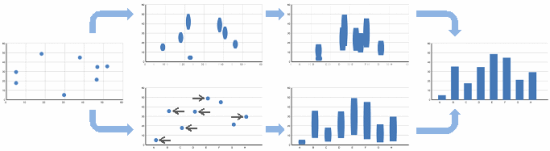
\includegraphics[width=0.8\textwidth, keepaspectratio]{images/methods/related/dynavis.png}
\caption[
    DynaVis \iacite{Heer2007}
]{DynaVis}
\label{fig:dynavis}
\end{figure}




% Die Forschungsarbeit war die erste Arbeit, welche die Effizenz von animierten Transitionen zwischen üblichen statischen Datengrafiken untersucht hat. Die Forscher haben in diesem Werk eine Einteilung von Transitionstypen vorgenommen und für das Erstellen von animierten Transitionen Design-Regeln aufgestellt. Anhand dieser zwei Konzepte erstellten sie eine Software namens DynaVis, mit der verschiedene Übergänge zwischen Darstellungen möglich sind (siehe Abbildung \ref{figure:related-animated-transitions}). Die Informationen in den folgenden Absätzen stammen aus dem Werk \citereset\cite{Heer2007}.

% Ziel des Projektes war es, zu untersuchen, ob Betrachter und Betrachterinnen von Datengrafiken mit Hilfe von animierten Transitionen Beziehungen zwischen den Visualisierungen erkennen können und während des Überganges die Orientierung beibehalten können. Die Forscher haben festgestellt, dass Datengrafiken anhand von drei Aspekten analysiert werden können: Syntaktisch, semantisch und pragmatisch. Die Syntax gibt die tatsächliche visuelle Darstellung (Punkte, Säulen, Linien, Achsen, Beschriftungen) und die Komposition der Darstellung an. Die Semantik hat den Fokus auf die Bedeutung der Grafik anhand der darunterliegenden Daten und deren Beziehung zueinander. Der Pragmatik kümmert sich um die Nebenbedeutungen, welche über die Semantik und die Syntax hinausgehen. In dem Forschungsprojekt von \citereset\cite{Heer2007} wurde nur die Syntax und die Semantik behandelt.

% Für eine Transition können das semantische Model, das darzustellende Schema, die Datenitems und die visuellen Kanäle verändert werden. Durch Veränderung der oben genannten Elemente verändert sich auch die Syntax der Darstellung. Bei einer statischen Transition wird die Syntax direkt mit einer neuen Syntax ersetzt. Datenpunkte in einem Streudiagramm werden beispielsweise für ein Säulendiagramm direkt durch Säulen ersetzt. In Abbildung \ref{figure:related-animated-transitions} würde man somit die zwei mittleren Schritte auslassen. Für eine animierte Transition muss jedoch zwischen den syntaktischen Eigenschaften (Position, Form, uvm.) interpoliert werden, sodass die semantischen Änderungen am effektivsten dem Betrachter oder der Betrachterin übermittelt wird.

% Im Zuge des Forschungsprojektes entstand eine Einteilungen in verschiedene Transitionstypen, welche bei syntaktischen oder semantischen Operationen für Datengrafiken benötigt werden:
% \begin{enumerate}
% \item \textit{View Transformation}: Wenn z.B. Panning oder Zooming verwendet wird, dann wird der Blickwinkel auf die Visualisierung verwendet. Die Veränderung der Ansicht ist rein syntaktischer Natur.
% \item \textit{Substrate Transformation}: Diese Transformation ist vorhanden, wenn der Untergrund einer Visualisierung verändert wird, z.B. durch eine Achsenskalierung oder einen Fischaugen-Effekt\footnote{https://de.wikipedia.org/wiki/Fischaugenobjektiv}.
% \item \textit{Filtering}: Wenn eine Filterung der Datenitems stattfindet, dann werden Elemente zur Visualisierung hinzugefügt oder entfernt. Visuelle Encodierungen oder das Datenschema wird dabei nicht verändert, aber es könnte eine Achsenskalierung notwendig sein.
% \item \textit{Ordering}: Ordinale Datendimensionen werden hier räumlich neu angeordnet.
% \item \textit{Timestep}: Verändert die dargestellten Datenwerte, z.B. um die Daten in einem Liniendiagramm für das darauf folgende Jahr zu untersuchen. Eventuell muss auch hier eine Achsenskalierung stattfinden.
% \item \textit{Visualization Change}: Liegt vor wenn visuelle Mappings für die Daten verändert werden, z.B. die Farbpalette wird verändert oder der Visualisierungstyp wird geändert.
% \item \textit{Data Schema Change}: Wenn beispielsweise von einem univariatem Säulendiagramm in ein bivariates Streudiagramm gewechselt werden soll, dann ändert sich das anzuzeigende Datenschema.
% \end{enumerate}

% Für alle oben genannten Übergänge galt es geeignete animierte Transitionen zu erstellen. Hierfür wurden noch Design-Prinzipien zum Erstellen von animierten Transitionen definiert. Diese Prinzipien können den zwei Hauptpunkten \textit{Übereinstimmung} und \textit{Verstand} zugeordnet werden:

% \newpage
% \begin{itemize}
%     \item \textit{Congruence}:
%     \begin{itemize}
%         \item \textit{Maintain valid data graphics during transitions}: Um dem Betracher oder der Betrachterin dabei zu helfen, das mentale Modell der Datengrafik beizubehalten, sollten möglichst wenig unerwünschte Eigenschaften zu den einzelnen Elementen während der Transition hinzugefügt werden z.B. unnötige Bewegung.
%         \item \textit{Use consistent semantic-syntactic mappings}: Ähnliche semantische Operatoren oder Änderungen sollen ähnliche animierte Transition erhalten.
%         \item \textit{Respect semantic correspondence}: Die Syntax sollte die Semantik nicht verletzten, da ansonsten Fehlinterpretationen getätigt werden können. Ein Datenpunkt soll beispielsweise immer die gleichen Daten repräsentieren.
%         \item \textit{Avoid ambiguity}: Im Idealfall sollte jeder semantische Operator oder jede Änderung eine unterschiedliche Transition erhalten, sodass man einen klaren Unterschied zwischen den Aktionen erkennen kann.
%     \end{itemize}
%     \item \textit{Apprehension}:
%     \begin{itemize}
%         \item \textit{Group similar transitions}: Die Elemente, auf die zur gleichen Zeit die gleiche Änderung wirkt, sollten möglichst so animiert werden, dass diese als Gruppe identifiziert werden können.
%         \item \textit{Minimize occlusion}: Objekte der Visualisierung sollten sich möglicht wenig überlappen, da ansonsten die Übersicht gefährdet ist.
%         \item \textit{Maximize predictability}: Sollte man nur einen Teil der Flugbahn eines Elementes beobachtet haben und weiß dann aber schon wo dessen Ziel ist, dann entlastet das und hilft beim Verstehen von Zusammenhängen.
%         % TODO später als Argument verwenden
%         \item \textit{Use simple transitions}: Die Flugbahn von animierten Elementen sollte möglichst einfach und nicht willkürlich sein, da ansonsten der Betrachter oder die Betrachterin eher überfordert ist, z.B. beim Verfolgen der Flugbahn von Elementen.
%         \item \textit{Use staging for complex transitions}: Um komplexe Transitionen besser wahrnehmen zu können, sollten sie in einzelne kürzere Subtransitionen unterteilt und anschließend seriell ausgeführt werden.
%         \item \textit{Make transitions as long as needed, but no longer}: Transitionen sollten nur so lange sein, dass der Betrachter oder die Betrachterin Elemente gut verfolgen kann. Dauern Transitionen zu lange, dann könnte das Engagement der Person beim Betrachten oder Verfolgen erheblich sinken.
%     \end{itemize}
% \end{itemize}

% Das für die Forschungsarbeit erstellte Programm DynaVis wurde mit der Programmiersprache C\# umgesetzt. Die animierten Transitionen werden so ausgeführt, dass die Animationsgeschwindigkeit erst beschleunigt und kurz vor dem Ziel wieder entschleunigt (im Englischen auch \textit{slow-in slow-out} Timing). Wenn in DynaVis gefiltert wird, dann werden die Elemente mit Hilfe von Alpha-Blending langsam ein- und ausgeblendet. Die Entwickler wollen so vermeiden, dass z.B. in einem Säulendiagramm eine Säule von oben in die Visualisierung herabfällt und der Betrachter oder die Betrachterin durch diese grundsätzlich bedeutungslose Bewegung falsche Rückschlüsse zieht. Werden die Elemente in der Visualisierung sortiert, dann werden diese nicht gleichzeitig, z.B. von einer Position zur anderen, sondern leicht versetzt animiert. So wird verhindert, dass sich mehrere Elemente während der Bewegung überlappen. DynaVis animiert auch Achsen und deren Beschriftungen. Die Achsen werden je nach Bedarf skaliert und die Achsenbeschriftungen werden sanft ein- und ausgeblendet. Wenn Eigenschaften wie z.B. Größe und Position für die nächste Visualisierung animiert werden müssen, dann wird darauf geachtet, dass z.B. erst die Position und dann die Größe animiert wird, sodass während der Positionsveränderung der Elemente möglichst wenig Überlappungen entstehen.

% Nach der Umsetzung von DynaVis wurde eine Benutzerstudie mit 24 Leuten durchgeführt. Diese nahmen an einer Serie von Tests teil. Ein Test beispielsweise beinhaltete Zielobjekte von einem in das nächste Diagramm zu verfolgen und dieses nach der animierten Transition zu lokalisieren. Auch gab es Aufgaben, bei denen die Probanden Größenveränderungen abschätzen mussten, z.B. nach einer Bewegung und Veränderung einer Säule in einem Säulendiagramm in ein gestapeltes Säulendiagramm. Das subjektive Feedback für die animierten Transitionen in DynaVis war von den meisten Propanden sehr positiv und viele wünschten sich die Verwendung dieser Art von Übergängen auch in alltäglichen kommerziellen Produkten.

% Das Ergebnis der Studie war, dass Animationen die grafische Wahrnehmung verbessern und bei der syntaktischen und schemantischen Analyse helfen. Gestaffelte Animationen wurden gegenüber den direkten Animationen meistens noch mehr bevorzugt, wobei hier galt, dass gestaffelte Animationen wirklich nur einen Schritt nach dem anderen animieren.